\section{Введение}
\subsection{Полнота пространств $L_p$}

\noindent

$(X, \MM, \mu)$ ~---~ пространство с мерой.

$p \in [1, +\infty]$

$\widetilde L_p (\mu)$  ~---~ полунормированное линейное пространство. Лишь \textit{полу}нормированное потому, что равенство 0 интеграла в $p$-ой степени от функции не означает равенство 0 этой функции, а лишь равенство этой функции нулю почти всюду.

$L_p (\mu)$ ~---~ нормированное линейное пространство.

Это всё было в прошлом семестре, теперь же мы докажем полноту пространства $L_p$.

\begin{reminder}
    Последовательность $\{ x_{n} \}$ называется \textit{фундаментальной}, если выполнено \textit{условие Коши}:
$$ \forall \epsilon > 0 \  \exists N (\epsilon) \in \N: \forall n \geq N, \forall m \geq N \hookrightarrow |x_{n} - x_{m}| < \epsilon. $$
\begin{enumerate}
    \item Каждая сходящаяся последовательность является фундаментальной, но не каждая фундаментальная последовательность сходится к элементу из своего пространства.
    \item Метрическое пространство, в котором каждая фундаментальная последовательность сходится к элементу этого же пространства, называется полным.
    \item \textit{Числовая} последовательность сходится тогда и только тогда, когда она фундаментальна.
\end{enumerate}

\end{reminder}

\begin{definition}
	Пусть $E = (E, \|\cdot\|)$  ~---~ линейное нормированое пространсвто (л.н.п.) Оно называется \textit{полным}, если
	
	$\forall$ фундаментальная (по норме $\|\cdot\|$) последовательность $\{x^n\}$ пространства $E$ сходится по норме пространства $E$ к некоторому элементу $x \in E$.
\end{definition}

\begin{definition}
	Дано $E = (E, \|\cdot\|)$  ~---~ л.н.п. Пара последовательностей $\{x^n\}_{n=1}^{\infty}$ и $\{S^k\}_{k=1}^\infty$, где \[
		S^k := \sum_{n=1}^k x^n ,
	\]
	называется формальным рядом в $E$. При этом $\{S^k\}_{k=1}^\infty$ называется последовательностью частичных сумм ряда, а $\{x^n\}_{n=1}^{\infty}$ ~---~ членами ряда. Часто пишут просто \[
		\sum_{k=1}^{\infty} x^k\text{ ~---~ формальный ряд.}
	\]
\end{definition}
\begin{note}
	В определении выше ряд мы называем \textit{формальным} потому, что ещё не было ничего сказано про его сходимость.
\end{note}
\begin{definition}
	Ряд $\sum\limits_{k=1}^\infty x^k$ называется сходящимся в л.н.п. $E$, если \[
	\exists x \in E:\; \left\|x - \sum_{k=1}^n x^k \right\| \ra 0, n \ra \infty
	\]
\end{definition}

\begin{definition}
	Ряд $\sum\limits_{k=1}^\infty x^k$ называется абсолютно сходящимся в л.н.п. $E$, если:\[
		\sum_{k=1}^{\infty} \|x^k\| \text{ ~---~ сходится}
	\]
\end{definition}


\begin{theorem}
	(Критерий полноты) $E$ ~---~ л.н.п. полно $\Longleftrightarrow\; \forall$абсолютно сходящийся в $E$ ряд является сходящимся.
\end{theorem}
\begin{proof}\ \\
	$(\implies)$\\

    Пусть $E$ полно и $\sum\limits_{k=1}^\infty x^k$ ~---~ сходится абсолютно $\implies\; \sum\limits_{k=1}^\infty \|x^k\|$ ~---~ сходящийся числовой ряд, а значит последовательность частичных сумм фундаментальна: \[
			\forall \epsilon > 0\; \exists N(\epsilon) \in \N:\forall n,m \geq N(\epsilon) \emb \sum_{k=n}^{m} \|x^k\| < \epsilon.
		\]
		В силу неравенства треугольника: $\left\|\sum\limits_{k=n}^m x^k\right\| \leq \sum\limits_{k=n}^m \|x^k\| < \epsilon$. \\
		Тогда $ \{S^n\}_{n=1}^\infty$ ~---~ поседовательность частичных сумм исходной последовательности фундаментальна в $E$.\\
		Но $E$ ~---~ полно $\implies \exists x \in E: \|x - S^n\| \ra 0, n \ra \infty \implies$ ряд $\sum\limits_{k=1}^\infty x^k$ ~---~ сходится в $E$\\
	($\impliedby$)\\
		Пусть $\{x^n\}$ ~---~ фундаментальная последовательноть в $E$. Это означает, что
		\[\forall \epsilon > 0\; \exists N(\epsilon) \in \N: \forall n, m \geq N(\epsilon) \emb \|x^n - x^m\| < \epsilon.\]
		Берём $\forall k \in \N\quad \epsilon_k = 2^{-k}$.\\
		$\exists \{N_k\}$ ~---~ строго возрастающая последовательность натуральных чисел такая, что \[
			\forall k \in \N\; \forall n, m \geq N_k \emb \|x^n - x^m\| \leq 2^{-k}.
		\]
		Рассмотрим $\{x^{N_k}\}_{k=1}^\infty$ ~---~ подпоследовательность последовательности $\{x^n\}$.\\
		Возьмём $y_k := x^{N_{k+1}} - x^{N_k}\quad \forall k \in \N$. Положим $y_0 := x^{N_1}$.\\
		Рассмотрим формальный ряд $\sum\limits_{k=0}^\infty y_k$. В силу выбора подпоследовательности, если в качестве $n$ выбрать $N_k$, а в качестве $m$ выбрать $N_{k+1}$, то неравенство $\|x^n - x^m\| \leq 2^{-k}$ будет выполнено $\implies \|y_k\| \leq 2^{-k} \implies \sum\limits_{k=0}^\infty y_k$ абсолютно сходится в $E$.\\
		Но по условию доказываемого утверждения, любой \textit{абсолютно сходящийся в $E$} ряд \textit{сходится} в $E$, значит\\
		ряд $\sum\limits_{k=0}^\infty y_k$ сходится $\implies \exists x \in E: \left\|x - \sum\limits_{k=0}^l y_k\right\| \ra 0, l \ra \infty$.\\
		При этом \[
			\sum_{k=0}^l y_k = y_0 + y_1 + \dots + y_l = x^{N_1} + x^{N_2} - x^{N_1} + \dots + x^{N_{l+1}} - x^{N_l} = x^{N_{l+1}}.
		\]
		Объединив два последних результата, получим \[
			\exists x \in E: \left\|x - x^{N_l}\right\| \ra 0, l \ra \infty.
		\]
		В итоге доказали существование элемента $x \in E$ т.ч. к нему сходится подпоследовательности $\{x^{N_l}\}_{l=1}^\infty$.\\
		Теперь остаётся воспользоваться условием фундаментальности и получить сходимость всей последовательности.
		\[
			\forall \epsilon > 0\; \exists L \in \N: \forall l \geq L \emb \|x - x^{N_l}\| < \frac{\epsilon}{2}.
		\]\[
			\forall \epsilon > 0\; \exists M \in \N: \forall n, m \geq M \emb \|x^n - x^m\| < \frac{\epsilon}{2}.
		\]\[
			\forall \epsilon > 0\; \exists N := \max\{L, M\} \in \N: \forall n \geq N	 \emb \| x - x^n \| \leq \| x - x^{N_M}\| + \| x^{N_M} - x^n\| < \frac{\epsilon}{2} + \frac{\epsilon}{2} = \epsilon.
		\]
\end{proof}
\begin{theorem}
	Пусть $p \in [1, +\infty]$. Тогда $L_p(\mu)$ полно.\\
\end{theorem}
\begin{proof}
	Разберём случай $p \in [1, +\infty)$. В силу предыдущей теоремы достаточно доказать, что любой абсолютно сходящийся ряд в $L_p(\mu)$ сходится в $L_p(\mu)$.\\
	Пусть $\sum\limits_{k=1}^\infty f_k$ ~---~ абсолютно сходящийся ряд в $L_p(\mu)$.
	То есть $\sum\limits_{k=1}^\infty \|f_k\|_p$ сходится как числовой ряд. Определим $F_n := \bigg(\sum\limits_{k=1}^{N} |f_k|\bigg)^p$. Используя неравенство Минковского, покажем, что $F_n$ интегрируема: \[
		\forall N \in \N \emb \left(\int\limits_X F_n(x)d\mu(x)\right)^{1/p} = \left(\int\limits_X \bigg(\sum_{k=1}^{N} |f_k|\bigg)^p d\mu(x)\right)^{1/p} \leq \sum_{k=1}^N \|f_k\|_p \leq \sum_{k=1}^{\infty} \|f_k\|_p < +\infty.
	\]
	Тогда $\{F_N\}_{N=1}^\infty$ ~---~ монотонная (неубывающая) функциональная последовательность.
	\begin{reminder}
		Монотонность функциональной последовательности ~---~ это монотонность последовательность по $n$ при каждом фиксированом $x$.
	\end{reminder}
	Тогда по теореме Леви \[
	\exists \lim_{N\ra\infty}\left(\int\limits_X F_n(x)d\mu(x)\right)^{1/p} = \left(\int\limits_X \lim_{N\ra\infty} F_n(x)d\mu(x)\right)^{1/p}
	\]\[
	\implies \left(\int\limits_X \bigg(\sum_{k=1}^\infty |f_k|\bigg)^p d\mu(x)\right)^{1/p} \leq \sum_{k=1}^{\infty} \|f_k\|_p < +\infty.
	\]
	\[
		\implies \sum_{k=1}^\infty |f_k(x)| \text{ конечна при $\mu$-п.в. }x \in X.
	\]
	При фиксированном $x$ имеем $\sum\limits_{k=1}^\infty f_k(x)$ ~---~ обычный числовой ряд, а для него из абсолютной сходимости следует сходимость.
	\[
		\implies\text{ при $\mu$-п.в.} x \in X\quad \sum_{k=1}^\infty f_k(x) \text{  конечна.}
	\]
	Положим $F(x) := \sum\limits_{k=1}^\infty f_k(x)$, эта функция корректно определена $\mu$-п.в. При этом $\mu$ ~---~ полная мера (меру считаем полной, если не было оговорено обратного). \[
		F(x) = \lim_{n \ra \infty} \sum_{k=1}^{n} f_k(x), \text{ этот предел существует для $\mu$-п.в. } x\in X.
	\]
	Остаётся доказать, что $\left\|F - \sum\limits_{k=1}^n f_k \right\|_p \ra 0, n \ra \infty$. Обозначим $n$-ый член этой последовательности как $J_n$.
	% Тут -----------------------------
	\[
		J_n = \left( \int\limits_X \bigg|\sum_{k=n+1}^\infty f_k(x) \bigg|^p d\mu(x) \right)^{1/p}
		\leq 
		\left(\int\limits_X \bigg(\sum_{k=n+1}^\infty |f_k(x)| \bigg)^p d\mu(x)\right)^{1/p}
		\incirc{\leq}
	\]
	Рассмотрим сумму ряда, как предел:
	\[
		\sum_{k=n+1}^\infty |f_k(x)| = \lim_{m \ra \infty} \sum_{k=n+1}^m |f_k(x)|.
	\]
	Вспомним лемму Фату:
	\[
		\text{При $g_k \geq 0$ верно}\int\limits_X \lim_{k \ra \infty} g_k(x) d\mu(x)
		\le
		\lowlim_{k \ra \infty} \int\limits_X g_k(x) d\mu(x).
	\]
	Тогда по лемме Фату:
	\[
		\left(\int\limits_X \bigg(\sum_{k=n+1}^\infty |f_k(x)| \bigg)^p d\mu(x)\right)^{1/p}
		\incirc{\leq}
		\sum_{k=n+1}^{\infty} \left( \int\limits_X |f_k(x)|^p d\mu(x) \right)^{1/p} \ra 0, n \ra \infty.
	\]
	Итого $J_n \ra 0, n \ra \infty$.
\end{proof}
\subsection{Неполнота $RL_p$}

\begin{definition}
	Пусть $RL_p([a, b])$ ~---~ линейное пространство функций, $p$-ая степень модуля которых интегрируема по Риману.
\end{definition}
\begin{remark}
	С таким определением это не является нормированным пространством. Чтобы сделать его нормированным, нужно аккуратно ввести класс эквивалентности.
\end{remark}
\begin{theorem}
	Пространство $RL_p([a, b])$ неполно.
\end{theorem}
\begin{proof} \ \\ 
	Без ограничения общности, $[a, b] = [0, 1]$.
	
	Пусть $\epsilon \in (0, \frac{1}{2})$.
	
	Перенумеруем рациональные точки отрезка $[0, 1]$:\quad $\Q \cap [0, 1] = \{r_k\}$.
	
	\[
	G_n := \bigcup_{k=1}^n \Big(r_k - \frac{\epsilon}{2^{k+2}}, r_k + \frac{\epsilon}{2^{k+2}}\Big) \cap  [0, 1].
	\]\[
	G := \bigcup_{n = 1}^\infty G_n.
	\]
	\begingroup
	\renewcommand{\theequation}{\arabic{equation}}
	Тогда $\chi_{G_n}$ интегрируема по Риману по критерию Лебега, потому что как характеристическая функция объединения конечного набора интервалов, пересечённых с отрезком, она обладает конечным числом разрывов. Таким образом
	\begin{equation}
		\{\chi_{G_n}\} \subset RL_p([0, 1]).
		\label{rlp:gn_rlp}
	\end{equation}
	
	Докажем, что $\chi_G$ имеет множество точек разрыва положительной меры Лебега. Для этого рассмотрим $F = [0, 1] \setminus G$. Тогда $\chi_G(F) = 0$, но в то же время $\chi_G(\mathbb{Q} \cap [0, 1]) = 1$, а так как $\Q$ плотно в $\R$, во всех точках $F$ функция $\chi_G$ разрывна. При этом по счётной полуаддитивности меры Лебега $\LL^n(G) \leq \frac{1}{2}$, а значит $\LL^n(F) \geq \frac{1}{2} > 0$. Итак, $\chi_G$ разрывна на множестве $F$ положительной меры, итого
	\begin{equation}
		\chi_G \not\in RL_p([0, 1]).
		\label{rlp:g_nrlp}
	\end{equation}
	
	Введём обозначения \[
		E_k := \Big(r_k - \frac{\epsilon}{2^{k+2}}, r_k + \frac{\epsilon}{2^{k+2}}\Big) \cap  [0, 1].
	\]\[
		G_m^n := \bigcup_{k=n}^m E_k.
	\]
	(в новых обозначениях $G_n = G_n^1$)
	и покажем фундаментальность последовательности $\{\chi_{G_n}\}$:
	\[
		\int_{0}^{1} |\chi_{G_m}(x) - \chi_{G_n}(x)| dx
		= \text{так как $G_n \subseteq G_m$} =
		\int_{0}^{1} \chi_{G_m \setminus G_n}(x) dx
		\leq
		\int_{0}^{1} \chi_{G_m^n}(x) dx
		\leq
	\]\[
		\leq
		\sum_{k=n+1}^m \int_0^1 \chi_{E_k}(x) dx
		=
		\sum_{k=n+1}^m \frac{\epsilon}{2^k} \ra 0, \text{ при } n, m \ra \infty.
	\]
	\begin{equation}
		\text{Итого, последовательность }\{\chi_{G_n}\}\text{ фундаментальна в }RL_p([0, 1]).
		\label{rlp:fund}
	\end{equation}
	Как известно, $RL_p$ ~---~ подпространство $L_p$. Тогда, если у последовательности из $RL_p$ есть предел в $RL_p$, то он такой же и при рассмотрении её как последовательности в $L_p$ с пределом в $L_p$. В нашем случае, если бы у $\{\chi_{G_n}\}$ был предел в $RL_p([0, 1])$, то у неё был бы такой же предел в $L_p([0, 1])$. Но мы знаем, что её предел в $L_p([0, 1])$ это $\chi_G$, которая не лежит в $RL_p([0, 1])$. Значит, у $\{\chi_{G_n}\}$ нет предела в $RL_p([0, 1])$, однако это фундаментальная в $RL_p([0, 1])$ последовательность. Значит пространство $RL_p([0, 1])$ не полно.
	\endgroup
\end{proof}


\subsection{Функции ограниченной вариации}
\begin{definition}
	Пусть $T$ ~---~ разбиение отрезка $[a, b]$, т.е. \[
		T = \{x_i\}_{i=0}^{N_T}, \quad N_T \in \N
	\]\[
		a = x_0 < x_1 < \dots < x_{N_T} = b.
	\]
	Пусть $f: [a, b] \ra \R$. Тогда $V_T(f)$ ~---~ вариация функции $f$ по разбиению $T$\[
		V_T(f) := \sum_{k=0}^{N_T-1} |f(x_{k+1}) - f(x_k)|
	\]
	\[
		V_a^b(f) := \sup_{T\text{ - разбиение } [a, b]} V_T(f)
	\]
\end{definition}
\begin{definition}
	$f$ называется функцией ограниченной вариации на $[a, b]$, если\[
	V_a^b (f) < +\infty.
	\]
	Обозначается $f\in BV([a, b])$. От английского Bounded Variation.
\end{definition}
\begin{theorem}
	$BV([a,b])$ ~---~ линейное пространство.
\end{theorem}
\begin{proof} \ \\
	Покажем, что $f_1, f_2 \in BV([a, b]) \implies \alpha f_1 + \beta f_2 \in BV([a, b])$. Пусть $T$ ~---~ произвольное разбиение $[a, b]$. Тогда по неравенству треугольника \[
		V_T(\alpha f_1 + \beta f_2)
		\leq
		|\alpha| V_T(f_1) + |\beta| V_T(f_2).
	\]
	
	Взяв супремум по всем разбиениям [a, b] получим желаемое.
\end{proof}
\begin{lemma}
	Если $\forall f: [a, b] \ra \R$ монотонна на $[a, b]$, то $f \in BV([a, b])$ и её $V_a^b (f) = |f(b) - f(a)|$.
\end{lemma}
\begin{proof}
	Все $V_T(f) := \sum_{k=0}^{N_T-1} |f(x_{k+1}) - f(x_k)|$ одного знака, то есть модуль раскрывается одинаково, а тогда соседние слагаемые друг друга уничтожают.
\end{proof}
\begin{lemma}
	Пусть $-\infty < a < c < b < +\infty$. Тогда
	\[
	f \in BV([a, b]) \Longleftrightarrow \System{f \in BV([a, c]) \\ f \in BV([c, b])}.
	\]
	В случае, если $f \in BV([a, b])$, тогда \[
		V_a^b (f) = V_a^c (f) + V_c^b (f).
	\]
\end{lemma}
\begin{proof} \ \\
	\textbf{Шаг 1. } ($\implies$) и $\geq$\\
		
    Пусть $f \in BV([a, b])$. Обозначим:
    \begin{itemize}
        \item $T_1$ ~---~ произвольное разбиение $[a, c]$,
        \item  $T_2$ ~---~ произвольное разбиение $[c, b]$.
        \item $T = T_1 \cup T_2$ ~---~ разбиение отрезка $[a, b]$.
    \end{itemize}
    Тогда имеем, что  $V_{T_1}(f) + V_{T_2}(f) \leq V_T(f) \leq V_a^b (f)$.
    
    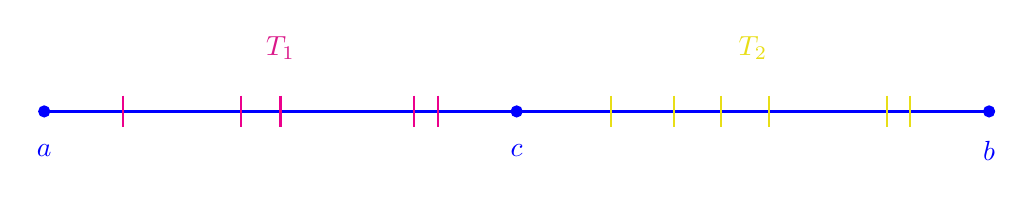
\begin{tikzpicture}
    
    % Основной отрезок
    \draw[thick, blue] (0,0) -- (12,0);
    
    % Точки alpha, c, beta
    \node[blue] at (0,-0.5) {$a$};
    \node[blue] at (6,-0.5) {$c$};
    \node[blue] at (12,-0.5) {$b$};
    
    \filldraw[blue] (0,0) circle (2pt);
    \filldraw[blue] (6,0) circle (2pt);
    \filldraw[blue] (12,0) circle (2pt);
    
    % Разбиение T1 на отрезке [alpha, c] (фиолетовые)
    \foreach \x in {1,2.5,3,4.7,5}
      \draw[magenta, thick] (\x,0.2) -- (\x,-0.2);
    
    % Разбиение T2 на отрезке [c, beta] (жёлтые)
    \foreach \x in {7.2,8, 8.6,9.2,10.7,11}
      \draw[yellow!90!black, thick] (\x,0.2) -- (\x,-0.2);
    
    % Подписи T1 и T2
    \node[magenta!90!black] at (3,0.8) {$T_1$};
    \node[yellow!90!black] at (9,0.8) {$T_2$};
    
    \end{tikzpicture} \\
    Взяв $\sup$ сначала по $T_1$, а потом по $T_2$, получим $V_a^c (f) + V_c^b (f) \leq V_a^b (f)$.
    
    \textbf{Шаг 2.} ($\impliedby$) и $\leq$ \\
    Пусть $\System{f \in BV([a, c]) \\ f \in BV([c, b])}$.\\
    Пусть $T = \{x_i\}_{i=0}^N$ ~---~ произвольное разбиение отрезка $[a, b]$.
    
    Если $c = x_{i^{*}}$ при некотором $i^{*}$, то это простой случай, так как тогда можно $\{x_j\}_{j=0}^{i^{*}}$ выбрать в качестве $T_1$, а $\{x_j\}_{j=i^{*}}^N$ выбрать в качестве $T_2$. И тогда очевидным образом $V_T(f) = V_{T_1}(f) + V_{T_2} (f) \leq V_a^c(f) + V_c^b (f) < +\infty$, а взяв $\sup$ по всем $T$ получим $V_a^b(f) \leq V_a^c(f) + V_c^b (f) < +\infty$.
    
    Теперь рассмотрим более интересный случай, когда ни при каком $i$ $x_i$ не равно $c$. Тогда $c \in (x_i, x_i + 1)$ при некотором $i$.
    \[\begin{aligned}
        V_T(f)
        & = \sum_{k=0}^{N - 1} | f(x_{k+1}) - f(x_k) | = \\
        & =
        \sum_{k=0}^{i - 1} |f(x_{k+1}) - f(x_k)| + |f(x_i) - f(x_{i+1})| +
        \sum_{k=i+1}^{N-1} |f(x_{k+1}) - f(x_k)| \leq \\
        & \leq
        \sum_{k=0}^{i - 1} |f(x_{k+1}) - f(x_k)| + |f(x_i) - f(c)| + |f(c) - f(x_{i+1})| +
        \sum_{k=i+1}^{N-1} |f(x_{k+1}) - f(x_k)|
        \incirc{\leq}
    \end{aligned}\]
    Обозначим разбиения:
    \begin{itemize}
        \item $T_1 = \{x_0, x_1, \dots, x_i, c\}$,
        \item $T_2 = \{c, x_{i+1}, \dots, x_N\}$.
    \end{itemize}
    Тогда полученный ранее результат можно оценить как
    \[
        \incirc{\leq} V_{T_1}(f) + V_{T_2}(f) \leq V_a^c(f) + V_c^b(f)
    \]
    Итого $V_T(f) \leq V_a^c(f) + V_c^b(f)$. Взяв $\sup$ по всем $T$, получим: \[
        \sup_T V_T(f) \leq V_a^c(f) + V_c^b(f)
    \]\[
        V_a^b(f) \leq V_a^c(f) + V_c^b(f)
    \]
    Если оба слагаемых в правой части конечны, то и $V_a^b$ конечна. Итого из первого и второго пункта \[
		V_a^b(f) = V_a^c(f) + V_c^b(f)
	\]
\end{proof}
Теперь воспользуемся этой леммой для доказательства следующей теоремы.
\begin{theorem}
	Пусть $f \in BV([a, b])$. Тогда функция $g(x) := V_a^x$ монотонно не убывает на $[a, b]$
\end{theorem}
\begin{proof}
	Пусть $x_2 > x_1$. Тогда применим только что доказанную лемму, выбрав $a = a, c = x_1, b = x_2$. \[
		V_a^{x_2} (f) = V_a^{x_1} (f) + V_{x_1}^{x_2} (f)
	\]\[
		V_a^{x_2} (f) - V_a^{x_1} (f) = V_{x_1}^{x_2}(f) \geq 0
	\]\[
		g(x_2) - g(x_1) \geq 0
	\]\[
		g(x_2) \geq g(x_1)
	\]
\end{proof}
\begin{theorem}
	Пусть $f \in BV([a, b])$. Тогда $\exists f_1$ и $f_2$ монотонно неубывающие на $[a, b]$ такие, что $f = f_1 - f_2$.
\end{theorem}
\begin{proof}
	Определим $f_1(x) := V_a^x(f) \quad \forall x \in [a,b]$. По только что доказанной теореме это монотонно неубывающая функция.\\
    	Докажем, что функция $f_2(x) = f_1(x) - f(x)$ монотонно не убывает.\[
		a \leq x \leq y \leq b.
	\]\[
		f_2(y) - f_2(x) = \bigg[f_1(y) - f(y)\bigg] - \bigg[f_1(x) - f(x)\bigg] = \bigg[f_1(y) - f_1(x)\bigg] - \bigg[f(y) - f(x)\bigg]
		\stackrel{(1)}{=} 
		V_x^y(f) - [f(y) - f(x)].
	\]
	(1) В силу аддитивности вариации по отрезкам\\
	Заметим, что $V_x^y(f) = \sup\limits_T V_T(f) \geq V_{\{x, y\}}(f) = |f(y) - f(x)|$. Тогда предыдущее выражение не меньше 0, а значит $f_2$ не убывает.
\end{proof}
\begin{corollary}
	$\forall f \in BV([a, b])$ имеет не более чем счётное множество точек разрыва, при том все они 1-го рода. (Из 1 семестра, помним что монотонная функция имеет не более чем счетное число точек разрыва, при том все они первого рода)
\end{corollary}

\subsection{Абсолютно непрерывные функции}

\begin{definition}
\label{def:ac}
	функция $f: [a, b] \ra \R$ называется абсолютно непрерывной на $[a,b]$, если

\begin{equation*}\begin{gathered}
	\forall \epsilon \; \exists \delta (\epsilon) > 0: \forall \text{ \underline{дизъюнктивной} системы }\{(a_k, b_k)\}_{k=1}^N:
	\sum_{k=1}^{N} |a_k - b_k| < \delta(\epsilon)
	\\
	\emb
	\sum_{k=1}^{n} |f(b_k) - f(a_k)| < \epsilon.
\end{gathered}
\end{equation*}
	$AC([a, b])$ ~---~ множество всех абсолютно непрерывных на $[a, b]$ функций.  От английского Absolutely Continuous.
\end{definition}
\begin{remark}
	$f \in AC([a, b])$ является непрерывной на $[a, b]$. (Так как из абсолютной непрерывности следует равномерная непрерывность.) Обратное неверно
\end{remark}
\begin{counterexample}
	\[
		f(x) = \begin{cases}
			x \sin\frac{1}{x}, & x \neq 0 \\ 0, & x = 0
		\end{cases}.
	\]
	$f \in C([0, 1])$, но $f \notin BV([0, 1])$, а значит по теореме, которая будет доказана ниже, $f \notin AC([0, 1])$.
\end{counterexample}
\begin{theorem}
	Если $f \in AC([a, b])$, то $f \in BV([a, b])$.
\end{theorem}
\begin{proof}
	Запишем \hyperref[def:ac]{определение абсолютной непрерывности} при $\epsilon = 1$. Тогда $\exists \delta = \delta(1) > 0: \forall$ конечного попарно непересекающегося набора интервалов $\{(a_k, b_k)\}_{k=1}^N: \sum\limits_{k=1}^{N} |b_k - a_k| < \delta \emb \sum_{k=1}^{N} |f(b_k) - f(a_k)| < 1$.\\
	Теперь разобъём отрезок $[a, b]$. Пусть $\N \ni M := \left[\frac{|b - a|}{\delta}\right] + 1$.
	\[\begin{aligned}
		&x_0 = a \\
		&x_1 = a + \frac{b - a}{M} \\
		&\vdots \\
		&x_M = a + b - a = b.
	\end{aligned}\]
	То есть поделили отрезок $[a, b]$ на одинаковые куски.\\
	Так как $x_{i+1} - x_i < \delta$ (специально для выполнение этого было взято достаточно большое $M$), то $\forall$ разбиение отрезка $[x_i, x_{i+1}]$ образует естественным образом конечным набор дизъюнктных интервалов суммарной длины меньше $\delta$, а значит по абсолютной непрерывности $V_{x_i}^{x_{i+1}}(f) < 1 \quad \forall i$\\
	Тогда в силу аддитивности вариации\\
	\[
		V_a^b(f) =
		\sum_{i=0}^{M-1} V_{x_i}^{x_{i+1}} (f)
		<
		\sum_{i=0}^{M-1} 1 = M < +\infty.
	\]
\end{proof}
